\section{Optimal Transport for Structured Data}
\label{sec:ot}

This section covers our works related to Optimal Transport distances for
structured data such as graphs.
In order to compare graphs, we have introduced the Fused Gromov Wasserstein
distance that interpolates between Wasserstein distance between node feature
distributions and Gromov-Wasserstein distance between structures.%
\cref{fn:titouan}
Here, we first introduce both Wasserstein and Gromov-Wasserstein distances and
some of our results concerning computational considerations related to the
latter.

\subsection{Wasserstein and Gromov-Wasserstein Distances}

Let $\mu = \sum_i h_i \delta_{x_i}$ and $\mu' = \sum_i h^\prime_i \delta_{x^\prime_i}$
be two
discrete distributions lying in the same metric space $(\Omega, d)$.
The $p$-Wasserstein distance is defined as:

\begin{equation}
    W_p(\mu, \mu') = \min_{\pi \in \Pi(\mu, \mu^\prime)}
        \left(\sum_{i,j} d(x_i, x^\prime_j)^p \pi_{i,j} \right)^{\frac{1}{p}}
    \label{eq:wass}
\end{equation}

where $\Pi(\mu, \mu^\prime)$ is the set of all admissible couplings between
$\mu$ and $\mu'$ (\emph{ie.} the set of all matrices with marginals $h$ and $h'$).%
\footnote{Note that the 2-Wasserstein distance is very similar in its formulation to
the Dynamic Time Warping similarity presented in Sec.~\ref{sec:dtw}.
The only difference lies in the constraints that are enforced in the
optimization problems.
For Wasserstein, a coupling needs to meet marginal constraints to be considered
valid while for Dynamic Time Warping, a path shall (i) not break the order of
the sequences at stake and (ii) enforce alignment of complete series (from
beginning to end).}
This distance is illustrated in Figure~\ref{fig:wass}.

\begin{figure}
\centering
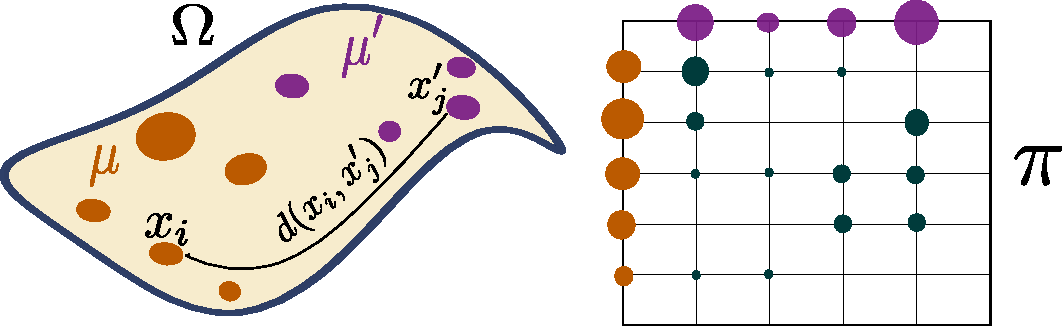
\includegraphics[width=.6\textwidth]{fig/wass}
\caption{Wasserstein distance. \label{fig:wass}}
\end{figure}

When distributions $\mu$ and $\mu'$ lie in distinct ambient spaces $\mathcal{X}$
and $\mathcal{X}^\prime$,
however, one cannot compute their Wasserstein distance. An alternative that was
introduced in~\cite{memoli2011gromov} relies on matching intra-domain
distances, as illustrated in Figure~\ref{fig:gw}.

\begin{figure}
\centering
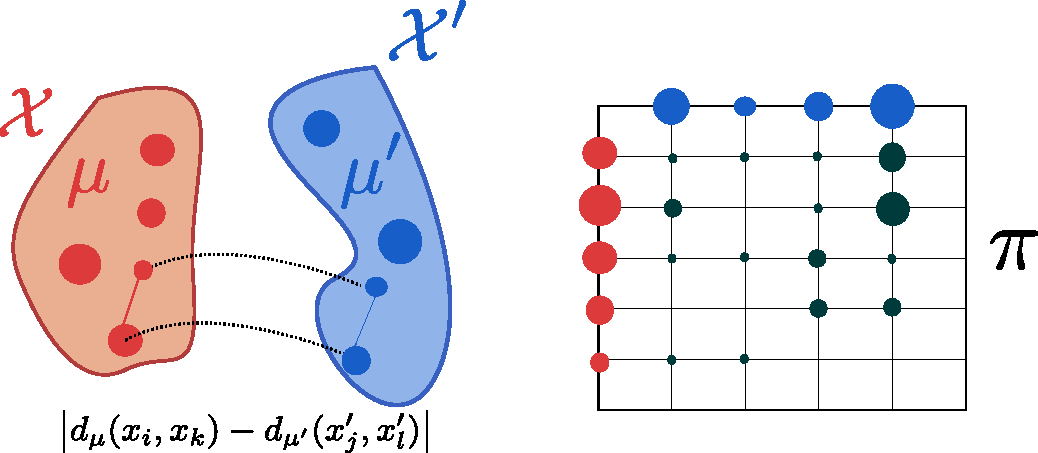
\includegraphics[width=.6\textwidth]{fig/gw}
\caption{Gromov-Wasserstein distance. \label{fig:gw}}
\end{figure}

The corresponding distance is the Gromov-Wasserstein distance, defined as:

\begin{equation}
    GW_p(\mu, \mu') = \min_{\pi \in \Pi(\mu, \mu^\prime)}
        \left(
            \sum_{i,j,k,l}
            \left| d_\mu(x_i, x_k) - d_{\mu'}(x^\prime_j, x^\prime_l) \right|^p
            \pi_{i,j} \pi_{k,l}
        \right)^{\frac{1}{p}}
    \label{eq:gw}
\end{equation}

\noindent
where $d_\mu$ (resp. $d_{\mu'}$) is the metric associated to $\mathcal{X}$
(resp. $\mathcal{X}^\prime$), the space in which $\mu$ (resp. $\mu'$) lies.

\subsection{Sliced Gromov-Wasserstein}

The computational complexity associated to the optimization problem in
Equation \eqref{eq:gw} is high in general.
However, we have shown in~\cite{vayer:hal-02174309} that in the
mono-dimensional case, this problem can be seen as an instance of the Quadratic
Assignment Problem~\cite{koopmans1957assignment}.
We have provided a closed form solution for this instance.
In a nutshell, our solution consists in sorting mono-dimensional distributions
and either matching elements from both distributions in order or in reverse
order, leading to a $O(n \log n)$ algorithm that exactly solves this problem.

Based on this closed-form solution, we were able to introduce a Sliced
Gromov-Wasserstein distance that, similarly to the Sliced Wasserstein
distance~\cite{rabin2011wasserstein}, computes similarity between distributions
through projections on random lines.

\subsection{Fused Gromov-Wasserstein}

Here, we focus on comparing structured data composed of a feature
and a structure information.
More formally, we consider undirected labeled graphs as tuples of the form $\mathcal{G}=(\mathcal{V},\mathcal{E},\ell_f,\ell_s)$ where
$(\mathcal{V},\mathcal{E})$ are the set of vertices and edges of the graph.
$\ell_f: \mathcal{V} \rightarrow \Omega_f$ is a labelling function that
maps each vertex $v_{i} \in \mathcal{V}$ to a feature
$a_{i} = \ell_f(v_{i})$ in some feature metric space
$(\Omega_f,d)$.
We will denote by \emph{feature information} the set of all the features
$(a_{i})_{i}$ of the graph.
Similarly, $\ell_s: \mathcal{V} \rightarrow \Omega_s$ maps a vertex $v_i$ from
the graph to its structure representation
$x_{i} = \ell_s(v_{i})$ in some structure space
$(\Omega_s,C)$ specific to each graph.
$C : \Omega_s \times \Omega_s \rightarrow \mathbb{R_{+}}$ is a symmetric
application which measures the similarity between the vertices in the
graph.
Unlike the feature space, however, $\Omega_s$ is implicit and in practice,
knowing the similarity measure $C$ is sufficient. With a slight abuse of
notation, $C$ will be used in the following to denote both the structure
similarity measure and the matrix that encodes this similarity between pairs of
nodes in the graph $\{C(i,k) = C(x_i, x_k)\}_{i,k}$.
Depending on the context, $C$ can either encode the neighborhood information of
the nodes, the edge information of the graph or more generally it can model a
distance between pairs of vertices such as the shortest path distance.
When $C$ is a metric, such as the shortest-path
distance, we naturally equip the structure with the metric space $(\Omega_s,C)$.
We denote by \emph{structure information} the set of all the structure
embeddings $(x_{i})_i$ of the graph.
We propose to enrich the previously described graph with a histogram which
serves the purpose of signaling the relative importance of the vertices in the
graph.
To do so, we equip graph vertices with weights $(h_{i})_{i}$ that sum to $1$.

All in all, we define \emph{structured data} as a
tuple $\mathcal{S}=(\mathcal{G},h_{\mathcal{G}})$ where $\mathcal{G}$ is a
graph as described above and $h_{\mathcal{G}}$ is a function that
associates a weight to each vertex. This definition allows the graph to be
represented by a fully supported probability measure over the product space
feature/structure $\mu= \sum_{i=1}^{|\mathcal{V}|} h_{i} \delta_{(x_{i},a_{i})}$, where
$\delta$ is the Dirac measure.
This probability measure
describes the entire structured data, as shown in Figure~\ref{fig:graph}.

\begin{figure}
\centering
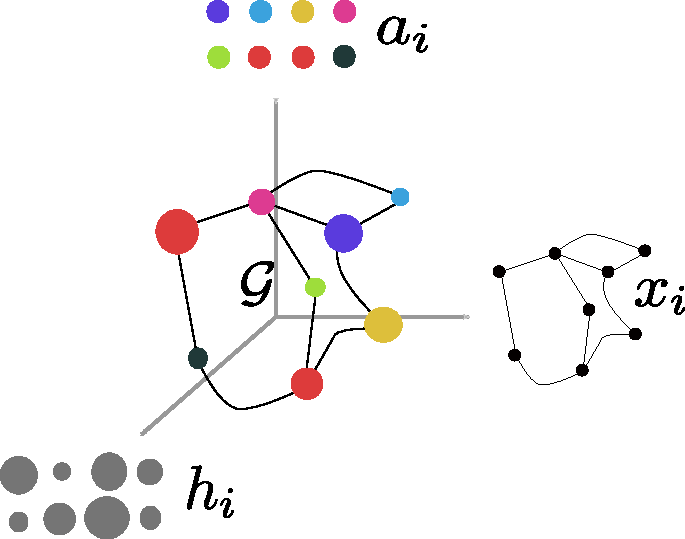
\includegraphics[width=.4\textwidth]{fig/graph_as_distrib}
\caption{A structured object can be described by a labelled graph with $(a_{i})_{i}$ the feature information of the object and $(x_{i})_{i}$ the structure information.
If we enrich this object with a histrogram $(h_{i})_{i}$ for measuring the relative importance of the nodes we can represent the structured object as a fully supported probability measure $\mu$ over the product space of feature and structure. \label{fig:graph}}
\end{figure}

\subsubsection{Distance Definition and Properties}

Let $\mathcal{G}$ and $\mathcal{G}'$ be two graphs with their respective weight
vectors $h$ and $h^\prime$, described respectively
by their probability measure $\mu= \sum_{i=1}^{|\mathcal{V}|} h_{i} \delta_{(x_{i},a_{i})}$
and $\mu' = \sum_{i=1}^{|\mathcal{V}^\prime|} h^\prime_i \delta_{(x^\prime_i,a^\prime_i)}$.
Their structure matrices are denoted $C$ and $C'$, respectively.


We define a novel Optimal Transport discrepancy which we call the
Fused Gromov-Wasserstein distance.
It is defined, for a trade-off parameter  $\alpha \in [0,1]$ and order $q$, as

\begin{equation}
\label{discretefgw}
FGW_{q, \alpha} (\mu, \mu') = \min_{\pi \in \Pi(\mu, \mu^\prime)}
    E_{q}(\mathcal{G}, \mathcal{G}', \pi)
\end{equation}

where $\pi$ is a transport map (\emph{i.e.} it has marginals $h$ and $h'$) and

\begin{equation}
E_{q}(\mathcal{G}, \mathcal{G}', \pi) =
    \sum_{i,j,k,l} (1-\alpha) d(a_{i},a^\prime_j)^{q}
                    +\alpha |C(i,k)-C'(j,l)|^{q} \pi_{i,j}\pi_{k,l} .
\end{equation}

The FGW distance looks for the coupling $\pi$ between vertices of the
graphs that minimizes the cost $E_{q}$ which is a linear combination of a cost
$d(a_{i},a^\prime_j)$ of transporting feature $a_{i}$ to $a^\prime_j$
and a cost $|C(i,k)-C'(j,l)|$ of transporting pairs of nodes in each structure.
As such, the optimal coupling tends to associate pairs of feature and
structure points with similar distances within each structure pair and with
similar features.
As an important feature of FGW, by relying on a sum of
(inter- and intra-)vertex-to-vertex distances, it can handle structured data
with continuous attributed or discrete labeled vertices
(depending on the definition of $d$) and can also be computed even if the graphs
have different numbers of nodes.

We have shown in~\cite{vayer:hal-02174322} that FGW holds the following
properties:

\begin{itemize}
\item it defines a metric for $q=1$ and a semi-metric for $q >1$;
\item varying $\alpha$ between 0 and 1 allows to interpolate between the
Wasserstein distance between the features and the Gromov-Wasserstein distance
between the structures;
\end{itemize}

In~\cite{vayer:hal-02174316},
we also define a continuous counterpart for FGW which comes with a
concentration inequality.
We present a Conditional Gradient algorithm for optimization on the
above-defined loss.
We also provide a Block Coordinate Descent algorithm to compute graph
barycenters \emph{w.r.t.} FGW, such as the ones presented in
Figure~\ref{fig:bary_fgw}.

\subsubsection{Results}

\begin{figure}
\centering
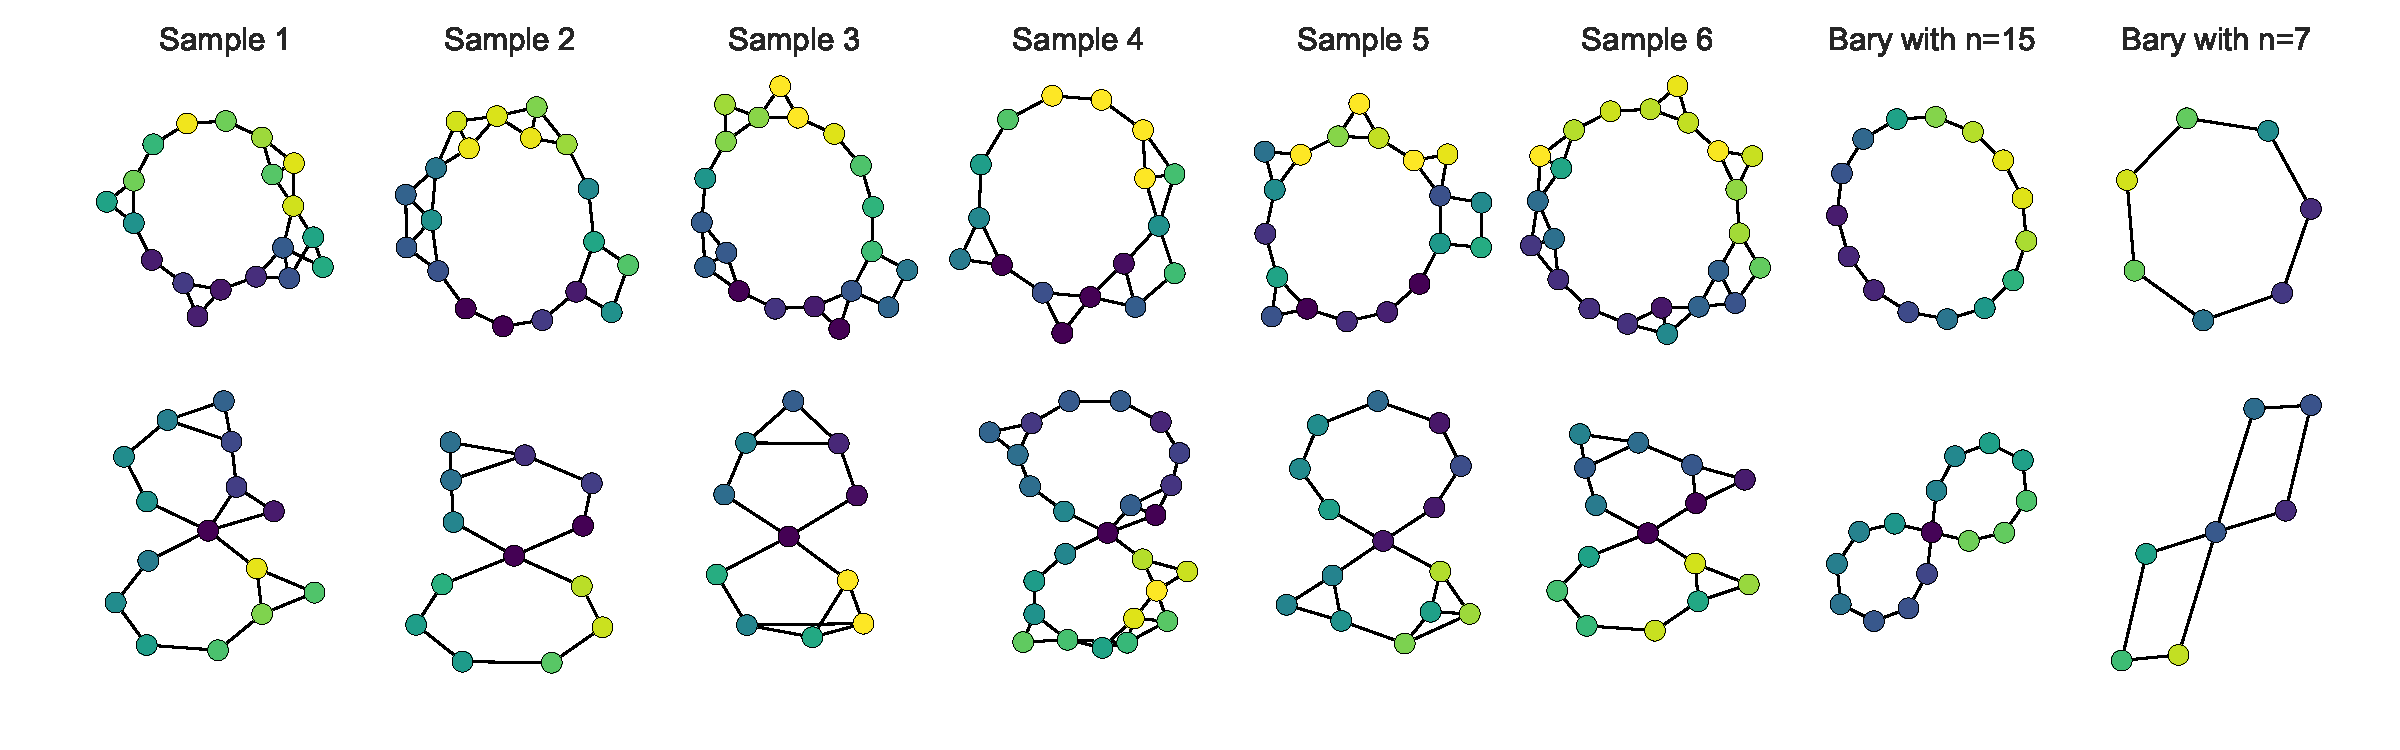
\includegraphics[width=\textwidth]{fig/fgw_bary}
\caption{Example barycenters computed using FGW as a metric for two datasets of
noisy labeled graphs. Node colors represent their mono-dimensional features and
barycenter structured is recovered by thresholding the structure matrix.
\label{fig:bary_fgw}}
\end{figure}

We have shown that such barycenters can be used for graph clustering.
Finally, we have exhibited classification results for FGW embedded in a
Gaussian-kernel SVM which leads to state-of-the-art performance
(even outperforming graph
neural network approaches) on a wide range of graph classification problems.
